% !Mode:: "TeX:UTF-8"

\chapter{绪论}

\section{课题研究的背景和意义}

随着计算机和软件技术的不断进步,软件系统的规模和复杂性也随之增长,尤其是那些被称为遗留
系统(legacy system)或遗产软件的项目。这些遗留系统由于其庞大的规模和维护升
级的难度,成为了代码质量分析的重要领域。根据 Chiu 等人的定义[1],遗留系统是指
那些维护和升级难度较高的大规模软件系统。而 Carvalho 等人[2]则将遗留系统描述为
依赖过时技术的系统,这些系统经过多年的广泛维护,导致其架构衰变和退化。遗留系
统的复杂性不仅体现在它们由紧密相连且相互依赖的组件构成,难以扩展和创新[3],还
在于它们对维护资源的巨大需求,这阻碍了数字化转型的步伐。尽管如此,这些系统代
表着长期的大规模投资,包含企业的重要数据和技术流程,完全抛弃可能会导致重要资
产流失,不可轻易放弃。因此,为了保持竞争力和保护现有投资,许多公司都选择对这
些遗留系统进行继续维护或者重构。

除了遗留系统之外,对于一般的软件项目,持续维护也是最重要的代码活动之一。调查显示,软件系统的维护成本在历年的软件维护预算中占 60\%到 80\%的比重[4]。标准的代码维护工作的流程图如图1-1所示,主要分为以下三个步骤:

(1)开发人员进行代码开发。修改项目代码后,针对修改部分进行回归测试,验证功能是否符合需求,同时避免缺陷的引入。

(2)测试通过后,由审查人员进行代码审查。代码审查的主要目的是确保代码质量,通过识别潜在的错误和优化点,提升代码的可维护性与可靠性,同时保证开发风格的统一。

(3)审查通过后,则可与原始项目进行合并。

\begin{figure}[h]
\centering
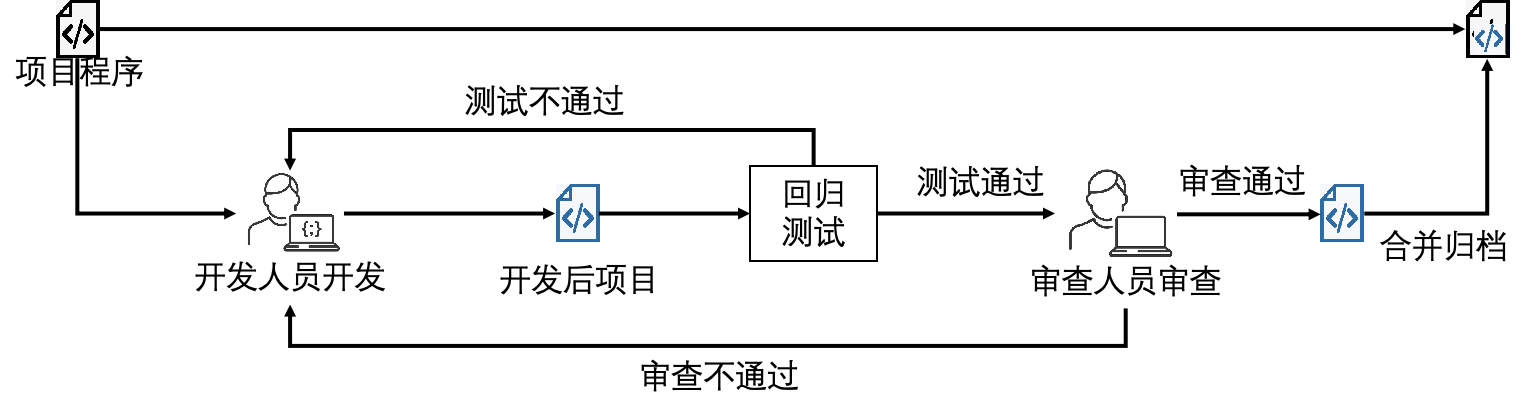
\includegraphics[width = 0.9\textwidth]{开发审查流程.png}
\caption{示例代码}
\end{figure}

软件项目由于历史原因,往往存在大量低质量代码和技术债务。在对软件项目进行维护或重构的过程中,代码质量分析是具有指导性意义的关键一环。代码质量分析可以帮助开发者识
别代码质量问题和问题所在的位置,提供有针对性的优化以及重构方案,从而降低成本和风险。通过有效的代码质量分析,企业可以逐步提升软件系统的稳定性和可维护性,为实现数字化转型打下坚实基础。这不仅能够保护企业的长期投资,还能提升整体竞争力,确保在快速变
化的市场中保持领先地位。

代码变更影响分析是代码质量分析的重要方法之一。通过代码变更影响分析,能够确定当某处代码进行变更时,系统中的其他哪些部分会受到影响,这可以让开发人员提前了解与变更部分有依赖关系的其他模块,避免变更时引入问题。

对于大型软件系统,代码变更影响分析更显得尤为关键。大型软件系统往往融合了不同开发者的个性化风格,随着时间的推移,系统的模块化设计原则逐渐被繁复和庞大的代码结构所淹没。这种情况下,精准地识别变更后有影响的代码模块,对于系统的有效重构和维护至关重要。然而,传统依赖经验丰富的专家
进行手工提取的方法,在面对日益复杂化的系统结构时,显得力不从心[5]。因此,从代
码变更影响分析的角度出发,不仅能深入理解代码变更对系统整体和各个子模块的潜在
影响,还能够提高维护项目的效率[6]。这种方法为软件系统的维护和升级提供了一种更
为科学和系统的解决策略,有助于实现软件质量的持续提升和维护成本的有效控制。

本文将从代码变更影响分析入手进行方法研究,面向代码质量评估,同时结合静态分析方法对代码项目进行代码度量提取和缺陷检测,帮助开发者和审查人员更直观地理解整个项目,为维护项目代码提供更有效的保障。

\section{国内外研究现状及分析}


\subsection{代码质量评估的国内外研究现状}

软件质量与软件的稳定性、可靠性、健壮性、可维护性等关键特性密切相关,是衡量软件性能和可靠性等指标的重要标准。作为软件质量的重要组成部分,代码质量在整体软件质量中占据着至关重要的地位,直接影响着软件系统的长期可用性与可维护性。

代码质量分析方法按照研究主题主要可以分为以下几种,

(1)代码缺陷

代码缺陷是研究最广泛的代码质量主题。相近地,代码漏洞、代码故障等概念也属于代码缺陷研究的范畴。软件代码中存在大量隐藏的缺陷,这些缺陷可能源于开发人员的疏忽、软件固有的逻辑漏洞或开发语言安全性的脆弱性。如果不进行及时的处理,这些问题可能引发安全漏洞,对系统和应用的安全造成影响。在此主题中,缺陷检测和预测是最主要的研究目的。

目前的研究方法主要分为三种,首先是传统的基于静态分析的方法,如基于代码相似度的检测器\cite{Sheneamer2018A,2014A}或基于模式的检测器\cite{2012Mitigating,2017IDE,2016How}。这种检测方法基于一系列预定义的规则、模式或静态模型进行检查,但是通常会产生较高的误报,检测的效果取决于预先定义的规则或模式的质量。其次是基于机器学习的方法。该种方法通过文本分析等方法提取代码特征,结合分类器,如决策树、支持向量机等机器学习技术\cite{2017Assessment,2018A,2020The},作为分类器,在大型数据集上进行预测。随着深度学习技术的发展,逐渐出现了基于深度学习技术的缺陷或漏洞预测方法,这种检测方法主要分为两步,首先通过代码表示学习方法,将代码表示为词嵌入、图表示或序列表示,利用神经网络捕捉代码语义和结构特征。通过端到端的深度学习模型直接从原始代码或中间表示中学习缺陷模式,训练模型后,直接对代码进行缺陷预测。


(2)代码复杂度

代码复杂度也是代码质量研究领域的重要主题之一。在\cite{NUNEZVARELA2017164}的研究中统计,代码复杂度在代码质量的主题中研究数量排在第二位。基于传统度量指标的研究通常是对经典复杂度度量的扩展,如在传统的度量标准,如圈复杂度、Halstead复杂度、CK度量的基础上,结合新型指标进行复杂度评估。除此之外,研究表示软件代码可以作为复杂网络来进行研究\cite{2015Exploring, 2012A},这类研究中通常将代码转化为图数据,如抽象语法树、调用图、控制流图、数据流图等,通过分析图结构的复杂性,捕捉代码逻辑的复杂程度。此外,基于认知复杂度也是代码复杂度的研究方法之一。认知复杂度衡量执行任务所需的人类努力\cite{2012Framework, 2012Asuite},是Shao和Wang\cite{2010Assessing}引入的认知指标的重要组成部分。这些度量标准与任何特定的编程范例都没有关联,但是可以从人因工程视角评估代码的认知复杂性,研究代码结构(如嵌套、条件分支)对开发者理解负担的影响,从而衡量代码的复杂性。


(3)代码内聚度和耦合性

内聚度和耦合性是软件设计中的核心指标,其平衡直接影响系统的质量与可维护性。高内聚度表示模块内部功能集中且相关性强,有助于提高代码的可读性和复用性,降低修改时的风险;低耦合性则强调模块间独立性,减少了相互依赖导致的连锁反应,使得系统更易于扩展和测试。二者共同作用,构成了高质量、易维护的软件架构的基础。

近年来对于内聚度的研究大多是从不同的角度提出新的度量标准,有少量研究是对传统度量指标的改进。\cite{陈振强2003}提出一种基于程序依赖性分析的类内聚度度量方法,它从属性与属性之间、属性与方法之间以及方法与方法之间三个方面对类进行全面分析.这三个方面既可以单独度量类的内聚度,也可以综合使用.证明了提出的方法满足Briand提出的关于优良的内聚度度量准则的四个基本性质。QU\cite{QU2015193}提出了两个新的类内聚度量MCC(Method Community Cohesion)和MCEC(Method Community Entropy Cohesion),这两种指标基于类中方法在不同社区间的分布,因此能够反映类的内聚程度。研究表明,这些指标可以提供现有类内聚性指标所未反映的额外且有用的信息。

同内聚度类似,对于耦合性的研究大部分也是对传统度量指标的改进。马健等人\cite{马健2018},参考 UML 中类图之间的关系,对 CBO (Coupling Between Object Classes)度量指标进行了改进,并使用一组形式化评估软件质量性质的定理进行评估; 以 JUnit 和 JEdit 为研究对象,对提出度量框架的关联、依赖、泛化关系进行度量研究。结果分析表明,改进后的指标可以较准确地反映面向对象设计中的耦合关系。


除此之外,还包括代码变更、代码可重用性、代码可读性、代码性能和代码安全性等研究主题。

根据不同的研究主题,演化出了很多代码度量套件,这些度量被广泛应用于与源代码相关的各种应用程序和实验中(例如,故障预测、测试、重构),以评估软件的整体质量。为了满足不同的度量需求,多年来,人们提出、研究和验证了许多来自不同编程范型的源代码度量,并不断提出新的度量和研究。研究发现\cite{Ardito2020},近年来使用最广泛的是Chidamber and Kemerer套件(CK套件)和Li and Henry(L&H)套件。



\begin{table}[htbp]
\caption{CK套件核心指标}
\vspace{0.5em}\centering\wuhao
\begin{tabular}{ccp{7.5cm}}
\toprule
度量 & 全称 & 描述 \\
\midrule
WMC & Weighted Methods per Class & 类中的方法的复杂性,复杂性可以通过方法数量或具体的计算方式(如方法的圈复杂度)来衡量 \\
DIT & Depth of Inheritance Tree & 类在继承树中的深度 \\
NOC & Number of Children & 一个类直接子类的数量 \\
CBO & Coupling Between Object Classes & 类与其他类之间的耦合关系数量  \\
RFC & Response for a Class & 类能够响应的所有方法的数量,包括其直接定义的方法和调用的其他类的方法  \\
LCOM & Lack of Cohesion in Methods & 类中方法间缺乏内聚性的程度  \\
\bottomrule
\end{tabular}
\end{table}

CK套件主要是针对面向对象语言设计的度量套件,具体含义如表1-1。CK套件中共有六个核心指标,侧重点各有不同,其中WMC用于衡量类的复杂性。如果值较高,说明类可能过于复杂,难以维护。DIT用于衡量类继承层次的复杂性。较大的DIT值表明更深的继承层次,增加了设计复杂性。NOC计算了一个类的直接子类的数量,衡量了类的影响范围,NOC值较高可能表明父类的职责过于泛化。CBO衡量了类间的依赖性。如果值较高,表示类之间耦合较强,模块化和重用性可能会较低。RFC衡量类的复杂性和可能的行为范围。RFC值较高可能表明类的行为过于复杂.LCOM衡量类内部方法和字段的相关性。如果值较高,说明类可能职责分散,应考虑拆分或重构优化。CK套件提供了一种系统化的方法来评估软件质量,能够帮助开发人员识别潜在问题,改进代码可维护性和可重用性。虽然CK套件主要是应用于面向对象语言的,但是也可应用于面向过程语言,只是需要根据具体场景调整权重和解释。

L\&H套件是由Li和Henry等人提出\cite{1993Object},主要用于评估程序的复杂度、维护性以及开发成本等度量套件。L&H套件中有一部分指标和CK套件是一样的,除此之外,还有另外五个核心指标。 

\begin{table}[htbp]
\caption{L\&H套件核心指标}
\vspace{0.5em}\centering\wuhao
\begin{tabular}{ccp{8cm}}
\toprule
度量 & 全称 & 描述 \\
\midrule
DAC & Weighted Methods per Class & 类之间通过抽象数据类型(Abstract Data Type)进行交互的程度 \\
MPC & Message Passing Coupling & 类之间通过方法调用进行通信的频率 \\
NOM & Number of Methods & 类中所有方法(包括继承和自定义方法)的数量 \\
SIZE2 & Second Order Size Metric & 通常用类的属性数和方法数的平方和表示  \\
SLOC & Source Lines of Code & 源代码行数  \\
\bottomrule
\end{tabular}
\end{table}

其中,较高的 DAC和MPC 值表示类对其他类的依赖程度较高,可能导致耦合度增加。较高的NOM和SIZE2 可能表明类的职责过多,过于复杂,难以理解和维护。较高的 SLOC 值表示代码较为冗长,可能需要优化。


\subsection{代码变更影响分析方法}


\section{本文的主要研究内容以及各章节安排}
\subsection{主要研究内容}
\subsection{章节安排}


